En este ejercicio, nos limitamos a pensar situaciones de la vida real que pudieran ser modeladas con $cliques\ de\ máxima\ frontera$.
\begin{itemize}

\item La conocida empresa internacional \textit{Chumbawamba} decide formar un equipo de trabajo para un proyecto que cambiará el mundo. Para que éste funcione sin peleas de por medio, dicho equipo debe consistir en un grupo de personas que se conozcan entre sí. Dado que la empresa desea que el proyecto sea conocido por la mayor cantidad de gente posible (siendo el boca en boca su única forma de difusión), deciden seleccionar a sus empleados de acuerdo a un conjunto que se conozca entre sí y que, también, conozca a la mayor cantidad de gente posible fuera de la empresa. Para modelar este problema, se consideran a los nodos como personas y a las aristas como la representación de un vínculo existente entre una persona y otra.
\begin{figure}[H] %[h] Aqui [b] para button [t] para top
\begin{center}
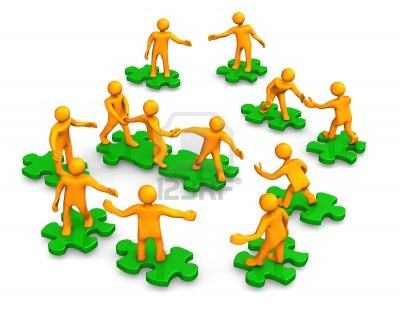
\includegraphics[width=250pt]{../imgs/ej1ejemp1.jpg}
\caption{Ejemplo}
\end{center}
\end{figure}

\item Un conocido golpeador desea asistir al recital de la mejor banda de todos los tiempos. Debido a su tardío horario de llegada al evento, éste se percata de que, desde el fondo del campo, lo único que puede visualizar es el cabello del de adelante. Bajo un ataque de furia decide comenzar a pegarle a la gente de forma estratégica para que, al tirar a una persona, se produzca un efecto dominó y se caigan todas las que se encuentran a menos de un metro y medio de ésta. De este modo, lograría tirar la mayor cantidad de gente al piso y disfrutar del recital tranquilo. Luego, nota que le conviene comenzar a golpear a las personas que se encuentran a menos de un metro y medio de distancia entre sí y que, además, se encuentran a menos de dicha distancia con la mayor cantidad de personas para que el alcance sea mayor. Para modelar este problema, consideramos a los nodos como personas y a las arista como la representación de que la distancia entre una persona y otra es menor a un metro y medio.  

 
\item En un campo casi como cualquier otro, se encuentran plantas que deben ser regadas con gran potencia para no morir. Debido a que, a medida que el agua atraviesa una planta, ésta pierde potencia, el granjero busca que la mayor cantidad de plantas sean regadas con alta potencia. Dado que el granjero es una persona de gran capacidad, decide armar una estrategia de riego para sus amadas plantas. Ésta consiste en encontrar qué planta regar para que se muera la menor cantidad de plantas. Para modelar este problema, se consideran a los nodos como plantas y a las aristas como caminos del sistema de riego por donde puede circular el agua. %no esta terminado

\item Virus distruibuido, quiero infectar la mayor cantidad de máquinas posible. la idea es que cuando ese virus se termina de ejecutar, infecta a todas las maquinas que estan conectadas a las que lo ejecutaron.

\end{itemize}
